
\newcommand\tr{\triangleright}
\newcommand{\proc}{\*{Proc}}
\newcommand{\bufst}{\*{BufState}}
\newcommand{\sups}{\*{Sups}}
\newcommand{\clis}{\*{Clis}}
\newcommand{\xducer}{\*{Xducer}}
\newcommand{\filling}{\texttt{Filling} \ }
\newcommand{\draining}{\texttt{Draining} \ }
\newcommand{\pin}{\texttt{Pin} \ }
\newcommand{\pout}{\texttt{Pout}}
\newcommand{\done}{\texttt{Done}}

\newcommand{\ftype}{\varphi}

\newcommand\mysnesl{SNESL\textsubscript{1}}

\def\interT#1#2{\vdash_{#1} #2}
\def\conc#1{#1 \ \underline{\mathtt{concrete}}}

\chapter{Implementation}

\def\Type#1#2#3{#1 \vdash_{\Sigma} \ #2 : #3 } 
\def\Eval#1#2#3{#1 \vdash_{\Phi} #2 \Eva #3 } 

In this chapter, we will first talk about the high-level interpreter of a minimal SNESL language but with the extension of user-defined functions to give the reader a more concrete feeling about SNESL. 
Then we introduce the streaming target language, SVCODE, with respect to its grammar, semantics and primitive operations.
Translation from the source language to the target one will be explained to show their connections.
Finally, two interpreters of SVCODE, an eager one and a streaming one, will be described and compared, with emphasis on the latter to demonstrate the streaming mechanism.



\section{High-level interpreter}


In this thesis, the high-level \mysnesl language we have experimented with is close to the SNESL introduced in the last chapter but without vectors, and we will call this language \mysnesl.
As our first goal is to extend SNESL with user-defined (recursive) functions,
it is safe to do so because removing vectors should not affect the complexity of the problem too much; we believe that if the solution works with streams, the general type in SNESL, it should work with vectors as well. 

Besides, only two primitive types of SNESL, $\int$ and $\bool$, are retained in \mysnesl. 
Tuples are also simplified to pairs.  

The types of \mysnesl \ are as follows.
\begin{align*} 
& \pi ::= \bool \ | \ \int \\
& \tau ::= \pi \ | \ (\tau_1,\tau_2) \ | \ \tseq{\tau}  \\
& \ftype :: = (\tau_1,...,\tau_k) \ra \tau 
\end{align*}

In \mysnesl, concrete types are either primitive types, or binary trees (i.e., nested pairs) of primitive types. 
We give its definition as follows:
\fig{
	\Jug{\conc{\tau}}
	
	\PT{\Axiom{\conc{\pi}}}
	\PT{\AC{\conc{\tau_1}}
		\AC{\conc{\tau_2}}
		\BC{\conc{(\tau_1,\tau_2)}}
}}{Concrete types}


The values in \mysnesl \ are:
\begin{align*}
& a ::=  \T \ | \ \F \ | \ n  \\
& v ::=  a \ | \ (v_1,v_2) \ | \ \{v_1,...,v_l\} 
\end{align*}

The abstract syntax of \mysnesl \ is given in Figure~\ref{fig-mysnesl}. 
 

\begin{figure}[H]\large
	\begin{alignat*}{2}
	& t &&::= e \ | \ d \ t  \tag{top-level term} \\
	\\
	& e &&::=  a \     \tag{constant} \\
	&   && \quad | \ x  \tag{variable} \\
	&   && \quad | \ (e_1,e_2) \tag{pair}\\
	&   && \quad | \ \{e_1,...,e_k \}_{\qquad k \ge 1}	\tag{primitive sequence} \\
	&   && \quad | \ \{ \}\tau			\tag{empty sequence of type $\tau$} \\
	&   && \quad | \ \Let{x}{e_1}{e_2} \tag{let-binding}\\
	&   && \quad | \ \hcall{\Tupk{e}}  \tag{built-in function call} \\
	&   && \quad | \ \Comp{e_1}{x}{e_0}{\usevarsk} \tag{general comprehension} \\
	&   && \quad | \ \RComp{e_1}{e_0}{\usevarsk} \tag {restricted comprehension} \\
	&   && \quad | \ f(e_1,...,e_k)  \tag {user-defined function call} \\
	\\
	& d &&::= \*{function} \  f(x_1: \tau_1, ..., x_k: \tau_k): \tau = e  \tag{user-defined function}
	\end{alignat*}
	\caption{Abstract syntax of \mysnesl \ \label{fig-mysnesl}}
\end{figure}

In addition to the simplifications mentioned before, we also made the following changes or extensions on expressions from SNESL:

\begin{itemize}
	\item For comprehension expressions, the free variables of the comprehension body $e_1$ are collected as a list added after the keyword $\*{using}$. This task can simply be done by the front end of the compiler; we do this for presenting the details of implementation more conveniently.
	
	\item Added primitive sequence expression (including the empty one with its type explicitly given). They work as a replacement of the function $\*{mkseq}$.
	
	\item Added user-defined functions which allow recursions. Since type inference is not incorporated in the interpreter, the types of  parameters and return values need to be provided when the user defines a function.
\end{itemize}


The typing rules for the expressions of \mysnesl \ are given in Figure~\ref{fig-snesl1-typing}. The type environment $\Gam$ is a mapping from variables to types: $$\Gamma = [x_1 \|-> \tau_1, ..., x_k \|-> {\tau_k} ]$$
and $\Sigma$ from the identifiers of user-defined functions  to their types: 
$$\Sigma = [f_1 \|-> \ftype_1,..., f_k  \|-> \ftype_k ]$$

\fig{
	\Jug{\Type{\Gam}{e}{\tau}}
	
	\PT{
		\RiLa{(\TypeV{a}{\pi})}
		\Axiom{\Type{\Gam}{a}{\pi}}
	}
	\PT{
		\AxiomC{}
		\RiLa{(\Gam(x) = \tau)}
		\UC{\Type{\Gam}{x}{\tau}}
	}\\[4ex]
	\PT{
		\AC{\Type{\Gam}{e_1}{\tau_1}}
		\AC{\Type{\Gam}{e_2}{\tau_2}}
		\BC{\Type{\Gam}{(e_1,e_2)}{(\tau_1,\tau_2)}}
	}\\[4ex]	
	\PT{
		\AC{\Type{\Gam}{e_1}{\tau}}
		\AC{...}
		\AC{\Type{\Gam}{e_l}{\tau}}
		\TC{\Type{\Gam}{\{e_1,...,e_l\}}{\{\tau\}}}
	}
	\PT{\Axiom{\Type{\Gam}{\{\}\tau}{\{\tau}\}}}
	\\[4ex]
	\PT{
		\AC{\Type{\Gam}{e_1}{\tau_1}}
		\AC{\Type{\Gam[x \|-> \tau_1]}{e_2}{\tau}}
		\BC{\Type{\Gam}{\Let{x}{e_1}{e_2}}{\tau}}
	}\\[4ex]
	\PT{
		\AC{\k{\Type{\Gam}{e_i}{\tau_i}} }
		\AC{\Typef {\hcall} {\replc{k}{\tau}} {\tau}}
		\BC{\Type{\Gam}{\hcall{\Tupk{e}}}{\tau}}
	}\\[4ex]	
	\PT{
		\AC{\Type{\Gam}{e_0}{\{\tau_0\}}}
		\AC{\Type{[x \|-> \tau_0, \k{x_i \|-> \tau_i}]}{e_1}{\tau}}
		\RiLa{(\k{\Gam(x_i) = \conc{\tau_i}})}
		\BC{\Type{\Gam}{\Comp{e_1}{x}{e_0}{\usevarsk}}{\tseq{\tau}}}
	}\\[4ex]
	\PT{
		\AC{\Type{\Gam}{e_0}{\bool}}
		\AC{\Type{[\k{x_i \|-> \tau_i}]}{e_1}{\tau}}
		\RiLa{(\k{\Gam(x_i) = \tau_i})}
		\BC{\Type{\Gam}{\RComp{e_1}{e_0}{\usevarsk}}{\tseq{\tau}}}
	}\\[4ex]
	\PT{
		\AC{\Type{\Gam}{e_1}{\tau_1}}
		\AC{...}
		\AC{\Type{\Gam}{e_k}{\tau_k}}
		\RiLa{(\Sigma(f) = (\tau_1, ... , \tau_k) \ra \tau)}
		\TC{\Type{\Gam}{f(e_1,...,e_k)}{\tau}}
	}

}{Typing rules of \mysnesl  \ expressions \label{fig-snesl1-typing}}


The typing rules for built-in operations (using the judgment $\boxed{\Typef {\hcall} {\replc{k}{\tau}} {\tau}}$) are given in their detailed descriptions later.


The typing rules of \mysnesl \ should be straightforward except those for comprehensions. 
For the general comprehension, the $input$ sequence $e_0$, as well as the whole expression, must be a sequence.
The types of the free variables of the $ comprehension \ body$ $e_1$, i.e., $x_1,...,x_k$, are all required to be concrete. That is, they cannot be sequences.
We will explain this later.
 
 
Figure~\ref{fig-snesl1-values} shows the typing rules for \mysnesl \ values, and Figure~\ref{fig:type-check} gives the rules for checking whether a top-level term is well-typed.

\fig{
\Jug{\TypeV{v}{\tau}}

\PT{\Axiom{\TypeV{n}{\int}}}
\PT{\Axiom{\TypeV{\T}{\bool}}}
\PT{\Axiom{\TypeV{\F}{\bool}}}\\[4ex]
\PT{
	\AC{\TypeV{v_1}{\tau_1}}
	\AC{\TypeV{v_2}{\tau_2}}
	\BC{\TypeV{(v_1,v_2)}{(\tau_1,\tau_2)}}
}
\PT{
	\AC{\TypeV{v_1}{\tau}}
	\AC{...}
	\AC{\TypeV{v_l}{\tau}}
	\TC{\TypeV{\{\replc{l}{v}\}}{\{\tau\}}}
}
}{Typing rules of \mysnesl \ values \label{fig-snesl1-values}}


\fig{
\Jug{\interT{\Sigma}{t}} \\
	\PT{
		\AC{\Type{[ \ ]}{e}{\tau}}
		\UC{\interT{\Sigma}{e}}
	}
	\PT{
		\AC{\Type{[x\|->\tau_1,..., x_k \|-> \tau_k]}{e}{\tau}}
		\AC{\interT{\Sigma[f \|-> (\tau_1,...,\tau_k) \ra \tau]}{t}}
		\BC{\interT{\Sigma}{\*{function} \  f(x_1: \tau_1, ..., x_k: \tau_k): \tau = e \ t}}
	 }
}{Well-typed top-level terms \label{fig:type-check}}

\hspace{1cm}

The semantics of \mysnesl \ is given in Figure~\ref{fig:mysnesl-semantics}. The evaluation environment  $\rho$ is in the form $$ \rho ::= [x_1 \|-> v_1,...,x_k \|-> v_k]$$ and the context for looking up user-defined functions $$\Phi ::= [f \|-> d_1,..., f_k\|-> d_k]$$

 %TODO: add cost??

\begin{figure}\large

 \Jug{\Eval{\rho}{e}{v}}
	 \PT{
	 	\Axiom{\Eval{\rho}{a}{a}}
	 }
	\PT{
		\AxiomC{}
		\RiLa{(\rho(x)=v)}
		\UC{\Eval{\rho}{x}{v}}
	}
	\PT{
		\AC{\Eval{\rho}{e_1}{v_1}}
		\AC{\Eval{\rho}{e_2}{v_2}}
		\BC{\Eval{\rho}{(e_1,e_2)}{(v_1,v_2)}}	
	}\\[4ex]
	\PT{
		\AC{\Eval{\rho}{e_1}{v_1}}
		\AC{...}
		\AC{\Eval{\rho}{e_l}{v_l}}
		\TC{\Eval{\rho}{\{e_1,...,e_l\}}{\{v_1,...,v_l\}}}	
	}
	\PT{
		\Axiom{\Eval{\rho}{\{\}\tau}{\{\}}}
	}\\[4ex]
	\PT{
		\AC{\Eval{\rho}{e_1}{v_1}}
		\AC{\Eval{\rho[x \|-> v_1]}{e_2}{v}}
		\BC{\Eval{\rho}{\Let{e_1}{x}{e_2}}{v}}	
	}\\[4ex]
	\PT{
		\AC{\k{\Eval{\rho}{e_i}{v_k}}}
		\AC{\hcall(v_1,...,v_k) \Eva v}
		\BC{\Eval{\rho}{\hcall{\Tupk{e}}}{v}}
	}\\[4ex]
	
	\PT{
		\AC{\Eval{\rho}{e_0}{\{v_1,...,v_l\}}}
		\AC{(\Eval{[x_1 \|-> \rho(x_1),...,x_k \|-> \rho(x_k), x \|-> {v_i},]}{e_1}{v_i'})^l_{i=1}}
		\BC{\Eval{\rho}{\Comp{e_1}{x}{e_0}{\usevarsk}}{\{\replc{l}{v'}}\}}
	}\\[4ex]	
	\PT{
		\AC{\Eval{\rho}{e_0}{\F}}
		\UC{\Eval{\rho}{\RComp{e_1}{e_0}{\usevarsk}}{\{\}}}
	}
	\PT{
		\AC{\Eval{\rho}{e_0}{\T}}
		\AC{\Eval{\rho}{e_1}{v_1}}
		\BC{\Eval{\rho}{\RComp{e_1}{x}{\usevarsk}}{\{v_1\}}}
	}\\[4ex]
	\PT{
		\AC{\k{\Eval{\rho}{e_1}{v_1}}}
		\AC{\Eval{[x_1 \|-> v_1,...,x_k \|-> v_k]}{e_0}{v}}
		\RiLa{\left(
			\begin{aligned}
			 \Phi(f)=  \*{function} \  & f(x_1: \tau_1, ..., x_k: \tau_k) \\
			 & : \tau = e_0
			\end{aligned}
		\right)}
		\BC{\Eval{\rho}{f{\Tupk{e}}}{v}}
	}\\
\caption{Semantics of \mysnesl \label{fig:mysnesl-semantics}}
\end{figure}

The evaluation rules are also straightforward except for the comprehensions.
In the general comprehension, the input sequence $e_0$ gets evaluated first, generating a sequence of $l$ elements.
These $l$ elements are used to substitute the bound variable $x$ in the comprehension body $e_1$; so $e_1$ will be evaluated $l$ times with different substitutions of $x$ but with the same value of its free variables $x_1,...,x_k$.
As mentioned before, these free variables $x_1,..., x_k$ can only be of concrete types, because their values are repeatedly used $l$ times here, which requires these values must be already materialized. 
If any of them is a stream, then there is no guarantee that this stream is already computed completely when the evaluation of $e_1$ starts, which may cause problems, such as a deadlock.

For the restricted comprehension, the $guard$ expression $e_0$ first gets evaluated: if it is a $\T$, $e_1$ will be evaluated, generating a singleton sequence; otherwise, $e_1$ will not be evaluated, and the comprehension only returns an empty sequence. \\


The built-in functions of \mysnesl \ correspond to a subset of SNESL's ones shown in Figure~\ref{fig-snesl-func} but without $\*{mqseq}$, $\*{zip}$ (can be desugared as nested pairs), and the vector-related ones. 
In addition, the function $\*{scan}$ and $\*{reduce}$ are also
taken a specific verison: picked $+$ from $\otimes$, for simplicity, as shown in Figure~\ref{fig-mysnesl-func}. 


\begin{figure}[H]\large
	\begin{alignat*}{2} 
	&\hcall && ::= \oplus \ | \  \ \*{append}_{\tau} \ | \ \*{concat}_{\tau}  \ | \ \*{iota}  \ | \ \*{part}_{\tau}  \ | \ \*{scan}_+ \ | \ \*{reduce}_{+} \ | \ \*{the}_{\tau}  \ | \ \*{empty}_{\tau} \\	
	& \oplus  \ && :: = + \ | \ - \ | \ \times \ |  \  / \ | \ \% \ | <= \ | \ == \ | \  \*{not} \ | \ ... \tag{scalar operations} 
	\end{alignat*}
	\caption{Primitive functions in \mysnesl \label{fig-mysnesl-func}}
\end{figure}

The types and semantics of these built-in functions remain the same as they are described in Table~\ref{tab:snesl-funcs}; we complement that brief version with more details where necessary and examples here.

\begin{itemize}

	\item $\*{append_{\tau} : \{\tau\} \times \{\tau\} \ra \{\tau\}}$ , 
	appends one sequence to the end of another; syntactic-sugared as the infix symbol {\++}.

	\begin{figure}[H]
	\begin{example}
	\end{example}
	\begin{lstlisting}[style = nesl-style]
	> {3,1} ++ {4}
	{3,1,4} :: {int}
	
	> {{3,1},{4}} ++ {{}int} ++ {{1,5}}
	{{3,1},{4},{},{1,5}} :: {{int}}
	\end{lstlisting}
	\end{figure}


	\item $\*{concat_{\tau}: \{\{\tau\}\} \rightarrow \{\tau\} }$, concatenates a sequence of sequences into one, that is, decreases the nesting-depth by one.
	\begin{figure}[H]
	\begin{example}
	\end{example}
	\begin{lstlisting}[style = nesl-style]
	> concat({{3,1},{4}})
	{3,1,4} :: {int}
	
	> concat({{{3,1}, {4}}, {{1}}})
	{{3,1},{4},{1}} :: {{int}}
	\end{lstlisting}
	\end{figure}

	\item $\*{iota: \int \ra \{\int\}}$, generates a sequence of integers starting from 0 to the given argument minus 1; syntactic-sugared as the symbol \&; if the argument is negative, then reports a runtime error.
	\begin{figure}[H]
	\begin{example}
	\end{example}
	\begin{lstlisting}[style = nesl-style]
	> &10
	{0,1,2,3,4,5,6,7,8,9} :: {int}
	
	> &0
	{} :: {int}
	\end{lstlisting}
	\end{figure}
	
	\item $\*{part_{\tau}: \{\tau\} \times \{\bool\} \ra  \{\{\tau\}\}}$, partitions a sequence into subsequences according to the second boolean sequence where a $\F$ corresponds to one element of the first argument and a $\T$ indicates a segment separation; so the number of $\F$s is equal to length of the first argument, and the number of $\T$s is equal to the length of the returned value, and this argument must end with a $\T$. 
	If the second argument does not satisfy these requirements, a runtime error will be reported.
	\begin{figure}[H]
	\begin{example}
	\end{example}
	\begin{lstlisting}[style = nesl-style]
	> part({3,1,4,1,5,9}, {F,F,T,F,T,T,F,F,F,T})
	{{3,1},{4},{},{1,5,9}} :: {{int}}
	
	> part({{3,1},{4},{}int, {1,5}}, {F,F,T,F,F,T})
	{{{3,1},{4}},{{},{1,5}}} :: {{{int}}}
	\end{lstlisting}
	\end{figure}
	
	\item $\*{scan_+}: \{\int\} \ra \{\int\}$, performs an exclusive scan of addition operation on the given sequence, that is, assuming the argument is $\{n_1,n_2,..,n_k\}$, to compute $\{0, n_1,n_1+n_2,...,n_1+...+n_{k-1}\}$. This scan operation has its general form in full SNESL, where it supports more associative binary operations with a specific identity element $a_0$  such that $a_0 \otimes a = a \otimes a_0 = a$ for all $a$.
	\begin{figure}[H]
	\begin{example}
	\end{example}
	\begin{lstlisting}[style = nesl-style]
	> scanPlus({3,1,4,1})
	{0,3,4,8} :: {int}
	
	> scanPlus({}int)
	{} :: {int}
	\end{lstlisting}
	\end{figure}
	
	\item $\*{reduce_+: \{\int\} \ra \int }$, performs a reduction of addition operation on the given sequence, i.e., computes its sum. 
	Again, this function also has its general form in full SNESL, where it computes $a_1 \otimes a_2 \otimes... \otimes a_k $ for an argument $\{a_1,a_2,...,a_k\}$.
	\begin{figure}[H]
	\begin{example}
	\end{example}
	\begin{lstlisting}[style = nesl-style]
	> reducePlus({3,1,4,1})
	9 :: int
	
	> reducePlus({}int)
	0 :: int
	\end{lstlisting}
	\end{figure}


	\item $\*{the_{\tau}:  \{\tau\} \ra \tau}$, returns the element of a singleton sequence; if the length of the argument is not exactly one, reports a runtime error. 
	\begin{figure}[H]
	\begin{example}
	\end{example}
	\begin{lstlisting}[style = nesl-style]
	> the({3})
	3 :: int
	
	> the({(3,1)})
	(3,1) :: (int,int)
	\end{lstlisting}
	\end{figure}
	
	\item $\*{empty_{\tau}:  \{\tau\} \ra \bool}$, tests if the given sequence is empty; if it is empty, returns a $\T$, otherwise returns a $\F$.
	\begin{figure}[H]
	\begin{example}
	\end{example}
	\begin{lstlisting}[style = nesl-style]
	> empty({3,1,4,1})
	F :: bool
	
	> empty({}int)
	T :: bool
	\end{lstlisting}
	\end{figure}
\end{itemize}



\section{Value representation} \label{sec:valrep}
At the low level, a value of \mysnesl \ is represented as either a primitive $stream$ (i.e., a collection of primitive values),
or a binary tree structure with stream leaves. 
The idea of this representation comes from \cite{Blel90vecmod}. 
The primitive stream $\a$ of $l$ elements $a_1,...,a_l$ and the stream tree $w$ have the following form: 
$$ \a ::= \<a_1,...,a_l\'>$$
$$ w ::= \a \ | \ (w_1,w_2) $$

The representation also relies on the high-level type of the value. 
We use the infix symbol ``$ \tr$" subscripted by a type $\tau$ to denote a type-depended representation relation.


\begin{itemize}
	\item A primitive value is represented as a singleton primitive stream: 
	\begin{example}
		$$3 \tr_\int \ \< 3 \'>$$
		$$ \T \tr_\bool \oT $$
	\end{example}
	
	
	\item A non-nested/flat sequence of length $n$ is represented as a primitive $data \ stream$ with an auxiliary boolean stream called a $descriptor$, which consists of $n$ number of $\F$s followed by one $\T$. 
	\begin{example}
		$$\{3,1,4\} \tr_{\{\int\}} (\< 3,1,4 \'>, \< \F, \F,\F , \T \'>) $$
		$$\{\T,\F\} \tr_{\{\bool\}} (\< \T,\F\'>, \< \F,\F , \T \'>) $$
		$$\{\} \tr_{\{\int \}} (\emptyv, \oT)$$
	\end{example}
	
	\item For a nested sequence with a nesting depth $d$ (or a $d$-dimensional sequence), all the data are flattened to a data stream, but $d$ descriptors are used to maintain the segment information at each depth. 
	(Thus a non-nested sequence is just a special case of $d$ = 1).
	
	\begin{example}
		$$\{\{3,1\}, \{4\}\} \tr_{\{\{\int\}\}} ((\< 3,1,4 \'>, \<\F,\F,\T,\F,\T \'>),\< \F, \F, \T \'>)  $$		
		$$\{\}\{\int\} \tr_{\{\{\int\}\}} ((\emptyv, \emptyv), \oT)$$
	\end{example}

	
	\item A pair of high-level values is a pair of stream trees representing the two high-level components respectively.  
	\begin{example}
		$$(1,2) \tr_{(\int,\int)} (\singl{1}, \singl{2})$$
		$$(\{\T,\F\},2) \tr_{(\{\bool\},\int)} ((\< \T, \F \'>, \< \F,\F,\T \'>),\singl{2})$$
	\end{example} 
	
	\item A sequence of pairs can be regarded as a pair of sequences sharing one descriptor at the low level:
	\begin{example}
		$$\{(1,\T),(2,\F),(3,\F)\} \tr_{\{(\int,\bool)\}} ((\<1,2,3\'>, \<\T,\F, \F\'>), \< \F,\F,\F,\T \'>)$$
	\end{example}
	
	
\end{itemize}


\section{SVCODE}
In \cite{Fmaster} a streaming target language for a minimal SNESL was defined.
With trivial changes in the instruction set, this language, named as SVCODE (Streaming VCODE), has been implemented on a multicore system in \cite{MF16}; the various experiment results
have demonstrated single-core performance similar to sequential C code for some simple 
text-processing tasks and near-linear scaling on modern	 multiple cores.

In this thesis, we put emphasis on the formalization of this low-level language's semantics.
Also, to support recursion in the high-level language at the same time preserve the cost, non-trivial extension of this language is needed. 

\subsection{SVCODE Syntax}

The abstract syntax of SVCODE is given in Figure~\ref{fig-svcode1-gram}.
An SVCODE program $p$ is basically a list of commands or instructions each of which defines one or more streams. 
We use $s$ to range over stream variables, also called stream $id$s, and $\S$ a set of stream ids.
As a general rule of reading an SVCODE instruction, the stream ids on the left-hand side of a symbol ``:=" are the defined streams of the instruction.


\begin{figure}[H] \large
	\begin{alignat*}{2}
	&p  && :: = \ \epsilon \tag{empty program}\\ 
	&   && \quad | \ \sdef{\s}{\psi(s_1,...,s_k)}  \tag{single stream definition}\\
	&   && \quad | \ \withctrl{\s}{p_1}{\Sin}{\Sout}  \tag{\wc block}\\
	&   && \quad | \ \scall{f}{s_1,...,s_k}{(s_1',...,s_{k'}')} \tag{SVCODE function call}\\
	&   && \quad | \ p_1;p_2  \\
	\\
	&\s && ::= 0 \ | \ 1 \ ... \in \SId  = \mathbb{N}   \tag{stream ids}\\
	&  \S && ::= \{\s_1,..., \s_k\} \in \sset  \tag{set of stream ids}\\
	\\
	& \psi \ && ::= \consta{a} \ | \ \toflag  
	\ | \ \usum \ | \ \map{\oplus} \ | \ \genscan_{\otimes} \ | \ \genreduce_{\otimes} \ | \ \distr  \tag{Xducers}  \\
    &   && \quad | \ \pack \ | \ \upack \ | \ \bu \ | \ \segconcat \ | \ \usegcount \ | \ \intermerge \ | \ ...  \\
    & \oplus  \ && :: = + \ | \ - \ | \ \times \ |  \  / \ | \ \% \ | <= \ | \ == \ | \  \*{not} \ | \ ... \tag{scalar operations} \\
    & \otimes \ && :: = + \ | \ \times  \ | \ ...  \tag{associative binary operations} \\
	\end{alignat*}
	\caption{Abstract syntax of SVCODE \label{fig-svcode1-gram}}
\end{figure}


The instructions in SVCODE that define only one stream are in the form
$$\sdef{\s}{\psi(s_1,...,s_k)} $$  
where $\lcall$ is a primitive function, called a \emph{Xducer}(transducer), taking the stream $s_1,...,s_k$ as parameters and returning \emph{s}. More detailed descriptions for specific Xducers are given in the next subsection.


The only essential control struture in this language is the \wc instruction 
$$\withctrl{\s}{p_1}{\Sin}{\Sout} $$
which may or may not execute a piece of SVCODE program $p_1$, but always defines a set of stream ids $\Sout$.
The definition instructions for all the stream ids in $\Sout$ are included in the code block $p_1$. 
Whether to execute $p_1$ or not depends on the value of the stream $\s$. We will call this special stream the $new \ control \ stream$, and we will give the explanation of the concept $control \ stream$ later, but here we only care about if $s$ is empty:
\begin{itemize}
	\item If $s$ is non-empty, then execute $p_1$ and generate the streams of $\Sout$ as usual
	\item Otherwise, skip $p_1$ and assign $\Sout$ all empty streams 
\end{itemize}
Thus the new control stream is the most important role here, because it decides whether or not to execute $p_1$, which is the key to avoiding infinite unfolding of recursive functions.  
$\Sin$ is a variable set including all the streams that are referred to by $p_1$;
it will only affect the streaming execution model of SVCODE, while in the eager model it can be ignored.

The instruction $\scall{f}{\replc{m}{s}}{(\replc{n}{s'})}$ can be read as: ``calling function $f$ with arguments $\replc{m}{s}$ returns $\replc{n}{s'}$". 
The function body of $f$ is merely another piece of SVCODE program, but without the definition instructions of its argument streams.


It is worth noting that a well-formed SVCODE instruction should always assign $fresh$ (never used) stream ids to the defined streams, in which way the dataflow of an SVCODE program can construct a DAG (directed acyclic graph). 
We will give more formal definitions of this language in the next chapter
to demonstrate how the freshness property is guaranteed. 
In the practical implementation, we simply identify each stream with a natural number, a smaller one always defined earlier than a greater one. 


\subsection{Xducers and control stream}

Transducers or Xducers are the primitive functions performing transformation on streams in SVCODE. 
Each Xducer consumes a number of streams and transforms them into another. 

For example, the Xducer $\map{+}(\<3,2\'>, \< 1,1\'>)$ consumes the stream $\<3,2\'>$ and $\< 1,1\'>$, then outputs 
the element-wise addition result $\<4, 3\'>$. 

\begin{example} \emph{$\map{+}(\<3,2\'>, \< 1,1\'>)$:}\\
	\begin{center}
		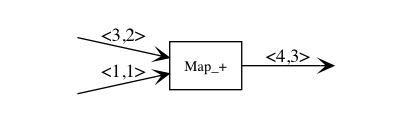
\includegraphics[width=0.6\textwidth]{fig/map.png}
	\end{center}
\end{example}


As we have mentioned before, the dataflow of an SVCODE program is a DAG, where each Xducer stands for one node. 
The \wc block is only a subgraph that may be added to the DAG at runtime,  
and \sc another that will be unfolded dynamically.

Figure~\ref{fig-svcode-eg1} shows an example program, with its DAG in Figure~\ref{fig-svcode-dag1}. \\

\begin{figure}[H]
	\begin{lstlisting}[style=svcode-style]
	S1 := Const_3();
	S2 := ToFlags(S1);
	S3 := Usum(S2);
	[S4] := WithCtrl(S3,[], 
	          S4 := Const_1();
	        )
	S5 := ScanPlus(S2, S4);
	\end{lstlisting}	
	\caption{A small SVCODE program \label{fig-svcode-eg1}}
\end{figure}
%	S6 := Usum(S2);
%	[S7] := WithCtrl(S6, [S5], 
%	[S7] := SCall(plus1, [S5])
%	)
\hspace{1cm}

\fig{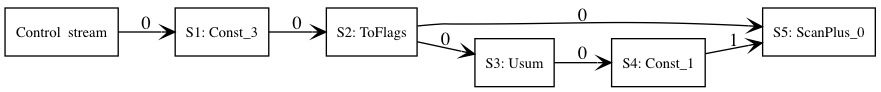
\includegraphics[width=1.1\textwidth]{fig/xducerDag2.png}}{
	Dataflow DAG for the code in Figure~\ref{fig-svcode-eg1} (assuming S3 is nonempty).
	\label{fig-svcode-dag1}
	Note that, for simplicity, the control stream is added as an explicit supplier only to Xducer $\consta{a}$.
}


When we talk about two Xducers $A$ and $B$ connected by an arrow from $A$ to $B$ in the DAG, we call $A$ a $producer$ or a $supplier$ to $B$, and $B$ a $consumer$ or a $client$ of $A$. 
As an Xducer can have multiple suppliers, we distinguish these suppliers by giving each of them an index, called a $channel \ number$. 
In Figure~\ref{fig-svcode-dag1}, the channel number is labeled above each edge. 
For example, the Xducer S2 has two clients, S3 and S5, for both of whom it is the No.0 channel;  Xducer S5 has two suppliers: S2 the No.0 channel and S3 the No.1. \\



Among all the Xducers, $\constaf{a}$ is a special one, because it outputs some number of constant $a$ but takes no argument.  
At the high level, it corresponds to the evaluation of constants.
Some strategy must be taken here to tell this Xducer how many elements it should produce.

In the implementation of \cite{MF16}, a special stream of unit type, called the $control \ stream$, is used at compiling time for replicating constants.

In our implementation, we move the control stream to the runtime, and let it not only control constants replication, but more importantly, dominate all the Xducers' behavior. 
Our observation is that the parallel degree throughout the whole computation can be expressed by this control stream, and all the Xducers can behave correspondingly to this parallel degree. 
So we make the Xducer read the control stream firstly before consuming its normal inputs, so that it will know how many elements it should read and output.

There are three benefits by doing so.

First, Xducers now can easily check a runtime error. 
For example, when the parallel degree is two, i.e., the control stream is $\< (),() \'>$, the Xducer $\map{+}$ will know that it only needs to consume two elements from each input stream, and output two as well; all the other cases will be reported as runtime errors.  
And the Xducer $\consta{a}$ just outputs the equal number of elements to the length of the control stream.

Another benefit is that all the Xducers will behave in a more uniform and regular way, which is easier for reason about and formalization, as we will show in the next chapter.

Finally, the functionality of the Xducer can be completely independent or separated from the scheduling (in the streaming execution model),  which makes the Xducer easier to be extended or changed,
and the implementation model more flexible and easier to debug. 



\section{Translating \mysnesl to SVCODE}
In Chapter~\ref{sec:valrep}, we have seen the idea of how a high-level value of \mysnesl \ can be represented as a binary tree of low-level stream values.
At the compiling time, we use a structure $\STree$ (stream id tree) to connect the high-level variables and the low-level ones: 
$$ \STree \ni \st ::= \s \ | \ (\st_1,\st_2) $$
The translation environment $\del$ is a mapping from high-level variables to stream trees:
 $$\del = [x_1 \|-> \st_1,..., x_k \|-> {\st_k}] $$ 

Another important component maintained at the compiling time is a fresh-stream allocation counter. 
It will be assigned to the defined stream(s) of the generated instruction by the translation.

We will use the symbol ``$\Ra$" to denote the translation relation. 
To avoid clutter, in this section we assume the defined stream id(s) of the new instructions are all fresh.

 
\subsection{Expression translation}


A \mysnesl \ expression will be translated to a pair of an SVCODE program $p$ and a stream tree $\st$ whose stream values represent the high-level evaluation result:
$$ \Trans{\del}{e}{}{}{\sfun{p}{\st}}$$

The translation for constants, variables and pairs are straightforward. For example, a pair $(x,4)$ will be translated to a program of only one instruction $s_0 := \constaf{4}$ and a stream tree $(s,s_0)$, assuming in the context $x$ is bound to $s$ and $s_0$ is a fresh id before the translation :   
$$[x \|-> \s] \Env (x,4)  \Ra (s_0 := \constaf{4}, (s,s_0))$$ 

For a let-binding expression $\Let{x}{e_1}{e_2}$,  first $e_1$ gets translated to some code $p_1$ with a stream tree $st_1$ as usual; then the binding $[x \|-> \st_1]$ is added to $\del$, in which the body $e_2$ gets translated to some $p_2$ with $\st_2$; the translation of the entire expression will be the concatenation of $p_1$ and $p_2$, i.e., $p_1;p_2$, and the stream tree is only $\st_2$.

Translations for specific built-in functions and user-defined functions will be given later.

%TODO explain or example
Non-empty primitive sequence looks a little bit tricky to translate as it can have arbitrary  number $n$ ($ n \ge$ 1) of elements, but it is basically a $n$-argument version of the function $\*{append}$.
For the empty sequence $\{\}\tau$, the low-level streams are all empty streams except for the outermost descriptor $\oT$, and the number of those empty streams depends on the type $\tau$.

The most interesting case may be the comprehensions. 
For the general one, $\Comp{e_1}{x}{e_0}{x_1,...,x_k}$, first we need to translate $e_0$, whose type must be a sequence, and we obtain a program $p_0$ and a stream tree that must look like $(st_0,s_b)$ where $s_b$ is the outermost descriptor. 
That is,
$$ \Trans{\del}{e_0}{}{}{(p_0,(st_0,s_b))}$$
Recall that the number of $\F$s of a descriptor is equal to the length of the inner data stream. 
We assume the length is $l$. 
The comprehension body $e_1$ will be evaluated $l$ times with $x$ being bound to different elements of the data stream $\st_0$, 
thus the parallel degree of computing $e_1$ will be $l$, and the control stream needs to be changed to represent the new parallel degree. 

Here we use the Xducer $\usum$ working on $s_b$ to generate the new control stream. The Xducer $\usumf{\b}$ consumes one boonlean stream and transforms an $\F$ to a unit, or a $\T$ to nothing.
\begin{example} \emph{$\usumf{\<\F,\T,\F,\F,\T\'>}$ with the control stream = $\<(),() \'>$:} \\
	\begin{center}
		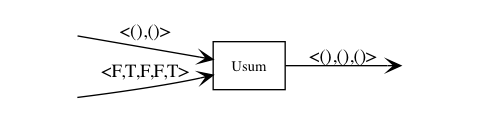
\includegraphics[width=0.6\textwidth]{fig/usum.png}
	\end{center}
\end{example}

If there is no free variables in $e_1$ (i.e., the list after $\*{using}$ is empty), then the next step of translating a general comprehension will be translating the comprehension body $e_1$ in the new environment $\del[x \|->\st_0]$, and the translation is finished.

For the case where $e_1$ uses some free variables $x_1,...,x_k$, we need to generate new streams, each of which is a $l$-replicate of the stream of $x_1,...,x_k$ respectively. 

So the translation will look like:\\[3ex]
	\PT{
		\AC{\Trans{\del}{e_0}{}{}{(p_0, (st_0,s_b))}}
		\AC{\Trans{[x \|-> {\st_0}, \k{x_i \|-> \st'_i}]}{e_1}{}{}{\sfun{p_1}{\st}}}
		\RiLa{(\k{\del(x_i) = \ \st_i})}		
		\BC{\Trans{\del}{\Comp{e_1}{x}{e_0}{\usevarsk}}{}{}
			{ \sfun{p} {(\st,\s_b)}}}
	}

\def\Distr#1#2#3{\mathtt{distr}_{#3}(#1,#2)}
\def\Pack#1#2#3{\mathtt{pack}_{#3}(#1,#2)}

in which $$ \begin{aligned}
p = ( & \ p_0; \\
    & \ \sdef{\s_1}{\usum(\s_b)}; \\
	& \ \sdef{\st_1'}{\Distr{\s_b}{\st_1}{\tau_1}}; \\
	& \qquad \qquad \vdots \\
	& \ \sdef{\st_k'}{\Distr{\s_b}{\st_k}{\tau_k}}; \\
	& \ \withctrl{\s_1}{p_1}{\Sin}{\Sout} ) \\
\end{aligned}$$	

Note that we put $p_1$ into a \wc block so that $p_1$ can be skipped when $s_1$, the new control stream, is tested to be an empty stream at runtime.
$\Sin$ and $\Sout$  are some analysis results about the free stream variables and the defined ones of $p_1$, which can be easily obtained by traversing $p_1$. We will give more details about them in the next chapter.

The function $\mathtt{distr}_{\tau}$ is responsible for replicating streams by using the Xducer $\distr$. 
We give its definition in a form close to the SVCODE style for more readability:
\begin{align*}
	s' := \Distr{s_b}{s}{\pi}; \quad \equiv & \quad s' := \distrf{s_b}{s}; \\
	(st'_1,st'_2)  := \Distr{s_b}{(st_1,st_2)}{(\tau_1,\tau_2)}; \quad \equiv & \quad st_1' := \Distr{s_b}{st_1}{\tau_1}; \\ 
	&\quad st_2' := \Distr{s_b}{st_2}{\tau_2};
\end{align*}

The Xducer $\distr$ consumes a boolean stream as a segment descriptor of the data stream, and replicates the constants of the data stream corresponding times to their segment lengths.
\begin{example} \emph{$\distrf{\<\F,\F,\F,\T,\F,\T\'>}{\< 2,5 \'>}$ with control stream $\< (),() \'>$}\\
	\begin{center}
		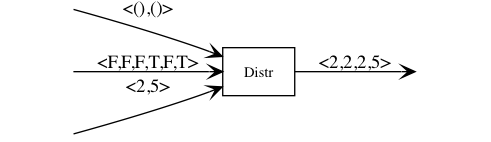
\includegraphics[width=0.7\textwidth]{fig/distr.png}
	\end{center}
\end{example}



The restricted comprehension is a little bit simpler compared to the general one, since there is no variable-bindings in $e_1$ and the parallel degree of the computation of $e_1$ is either one or zero, thus the free variables $x_1,...,x_j$ does not need to be distributed, but rather, $pack$ed. Its translation will look like:

$$\PT{
	\AC{\Trans{\del}{e_0}{}{}{(p_1,s_b)}}
	\AC{\Trans{[\j{x_i \|-> \st'_i}]}{e_1}{s_1}{}{\sfun{p_2}{\st}}}
	\RiLa{(\j{\del(x_i) = \ \st_i})}		
	\BC{\Trans{\del}{\RComp{e_1}{e_0}{\usevars}}{}{}
		{ \sfun{p} {(\st,\s_1)}}}
}$$


in which $$ \begin{aligned}
p = & \ p_1; \\
& \ \sdef{\s_1}{\bu(\s_b)}; \\
& \ \sdef{\s_2}{\usum(\s_1)}; \\
& \ \sdef{\st_1'}{\Pack{\s_b}{\st_1}{\tau_1}}; \\
& \qquad \qquad \vdots \\
& \ \sdef{\st_j'}{\Pack{\s_b}{\st_j}{\tau_j}}; \\
& \ \withctrl{\s_2}{p_2}{\Sin}{\Sout} \\
\end{aligned}$$
	
The Xducer $\bu$ simply transforms a boolean to a unary number, i.e.,  transforms $\oF$ to $\oT$, and $\oT$ to $\< \F, \T \'>$.
\begin{example} \emph{$\bu({\<\T,\F\'>})$ with control stream $\< (),() \'>$}\\
	\begin{center}
		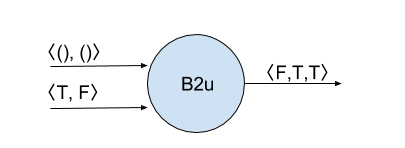
\includegraphics[width=0.6\textwidth]{fig/b2uxducer.png}
	\end{center}
\end{example}

The function $\mathtt{pack}_{\tau}$ annotated with the high-level type of the packed variable will generate instructions of $\pack$ and possibly $\upack$ and $\distr$:
\begin{align*}
s' := \Pack{s_b}{s}{\pi}; \quad \equiv & \quad s' := \packf{s_b}{s}; \\
\\
(st'_1,st'_2)  := \Pack{s_b}{(st_1,st_2)}{(\tau_1,\tau_2)}; \quad \equiv & \quad st_1' := \Pack{s_b}{st_1}{\tau_1}; \\ 
&\quad st_2' := \Pack{s_b}{st_2}{\tau_2};\\
\\
(st'_1,s_1')  := \Pack{s_b}{(st_1,s_1)}{\{\tau\}}; \quad \equiv & \quad s_1' := \upackf{s_b}{s_1}; \\ 
&\quad s_2' := \distrf{s_1}{s_b};\\
&\quad st_1' := \Pack{s_2'}{st_1}{\tau};
\end{align*}

The Xducer $\pack$ throws away the element of the second stream if the boolean of the corresponding position in the first stream is a $\F$. 

\begin{example} \emph{$\pack({\<\T,\F,\T\'>}, \<2,3,4 \'>)$ with control stream $\< (),(), () \'>$}\\
	\begin{center}
		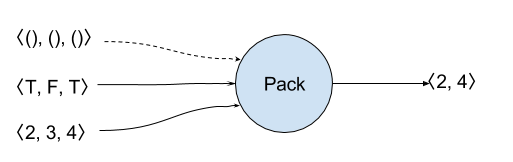
\includegraphics[width=0.6\textwidth]{fig/packxducer.png}
	\end{center}
\end{example}

$\upack$ works in a way similar to $\pack$, but on data of boolean segments rather than primitive values.
\begin{example} \emph{$\upack({\<\T,\F,\T\'>}, \< \F,\T,\ \ \F,\F,\T, \ \ \F,\F,\F, \T\'>)$ with control stream $\< (),(), () \'>$}\\
	\begin{center}
		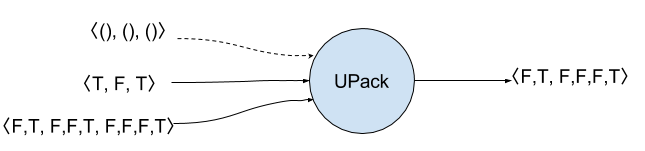
\includegraphics[width=0.8\textwidth]{fig/upackxducer.png}
	\end{center}
\end{example}


\subsection{Built-in function translation}
A high-level built-in function call will be translated to a few lines of SVCODE instructions.

\begin{itemize}
	\item Scalar operations, for instance $x_1 \oplus x_2$, will be translated to a single instruction $\map{\oplus}(s_1,s_2)$, assuming $\del(x_1) = s_1, \del(x_2) = \s_2$.
	
	\item The function $\iota{n}$  generates an integer sequence starting from 0 of length $n$.  
	The translation will first use the Xducer $\toflag$ to generate the descriptor of the return value, and then perform a scan operation on a stream of $n$ 1s to generate the data stream.
	Its translation will look like: 
	$$	\PT{
		\Axiom{\Transf{\iotan}{\s}{\s_0}{}{\sfun{p} {(\s_3,\s_0)}}}
	}$$
	where 
	\begin{align*}
			p= & \sdef{\s_0}{\toflag(\s)} ; \\ 
			& \sdef{\s_1}{\usum(s_0)} ; \\
			& \withctrl{\s_1}{\sdef{\s_2}{\consta{1}()}}{[]}{[\s_2]}; \\
			& \sdef{\s_3}{\scan_{0}(\s_0,s_2)}
		\end{align*}

Given a stream $\singl{n}$, the Xducer $\toflag$ first outputs $n$ $\F$s, then one $\T$.

\begin{example} \emph{$\toflagf{\<2,0\'>}$  with control stream $\<(),()\'>$:}\\
	\begin{center}
		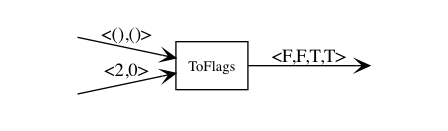
\includegraphics[width=0.6\textwidth]{fig/toflag.png}
	\end{center}
\end{example}

$\scan_{}(s_b,s_d)$ performs an exclusive scan on the data stream $s_d$ segmented by $s_b$.
\begin{example} \emph{$\scan_{}(\<\F,\F,\F,\T,\F,\T\'>, \< 2,5,3,6 \'>)$  with control stream $\<(),()\'>$: }\\
	\begin{center}
		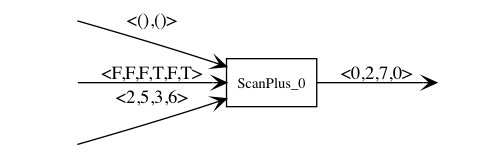
\includegraphics[width=0.7\textwidth]{fig/scan.png}
	\end{center}
\end{example}



\item The high-level function $\*{scan}_+$ is implemented straightforwardly by using the  Xducer $\scan_{}$:
	$$	\PT{
	\Axiom{\Transf{\*{scan}_+}{(s_d,s_b)}{\s_0}{}{\sfun{\sdef{s_0}{\scanf{s_b}{s_d}}} {(\s_0,\s_b)}}}
}$$

\item Translating $\*{reduce}_+$ is analogous to that of $\*{scan}_+$ by using its corresponding low-level Xducer $\mathtt{ReducePlus}$.

\item The translation of $\*{concat}$ is also one instruction using the Xducer $\segconcat$:
$$	\PT{
	\Axiom{\Transf{\*{concat}}{((st,s_1),s_2)}{\s_0}{}{\sfun{\sdef{s_0}{\segconcat(s_2,s_1)}} {(st,\s_0)}}}
}$$


The Xducer $\segconcat$ merges the second outermost descriptors of the high-level sequence, i.e., $s_1$, into a new one $s_0$ by removing unnecessary segment boundary $\T$s; the old outermost descriptor $s_2$ helps maintain the segmenting information.

\begin{example} \emph{$\segconcat(\<\F,\T,\F,\F,\F,\T\'>,\< \F,\T, \F,\F,\T,\T, \F,\F, \F,\T \'>)$ with control stream $\<(),()\'>$. The second argument has 4 segments, and the first argument says that the first one will be merged as one segment, and the other three together as another.}\\
	\begin{center}
		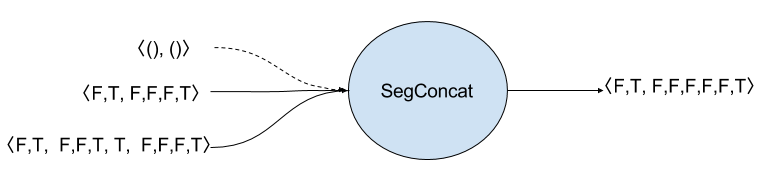
\includegraphics[width=0.9\textwidth]{fig/segconcatxducer.png}
	\end{center}
\end{example}


\item $\*{part}$ can be implemented straightforward by the Xducer $\usegcount$.
$$	\PT{
	\Axiom{\Transf{\*{part}}{(st_1,s_1),(s_2,s_2'))}{\s_0}{}{\sfun{\sdef{s_0}{\usegcount(s_2,s_2')}} {((\st_1,\s_2),s_0)}}}
}$$

$\usegcount$ counts the number of the segments of its second argument,  segmented according to the second argument, and represents it in unary.
\begin{example} \emph{$\usegcount(\< \F,\F,\F,\F,\F,\T,\F,\F, \F,\T \'>, \<\F,\T,\F,\F,\T,\F,\F,\T\'>)$ with control stream $\<(),()\'>$. The first argument indicates that the first 5 elements of the second argument are in the same segment, which has two $\T$s, and the last 3 another segment, which includes only one $\T$. So the unary form of the counting result (with segmenting) is $\<\F,\F,\T,\F, \T \'>$ }\\
	\begin{center}
		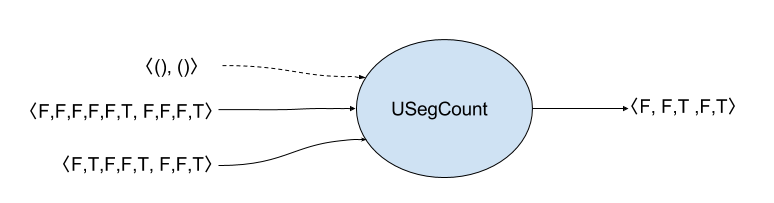
\includegraphics[width=0.9\textwidth]{fig/usegcountxducer.png}
	\end{center}
\end{example}


\item Implementation of the function $\*{append}$ may be the most tricky one, since it needs to recursively append subsequences at each depth of the argument sequences:
$$	\PT{
	\Axiom{\Transf{\*{append}}{(st_1,s_1),(st_2,s_2))}{\s_0}{}{\sfun{p} {(\st,\s_0)}}}
}$$
\def\mergeRecur#1{\mathtt{mergeRecur}_{#1}}
where 
\begin{align*}
p = & \ \sdef{\s_0}{\intermerge([s_1,s_2])} ; \\ 
    & \sdef{\st}{\mergeRecur{\{\tau\}}([(st_1,s_1),(st_2,s_2)])};
\end{align*}

The Xducer $\intermerge$ merges two descriptors by interleaving their segments. 
%TODO

The function $\mergeRecur{}$ annotated by the type of the argument merges the inner segments  recursively. 
Its definition is given below.

\begin{align*}
& s := \mergeRecur{\{\pi\}}([(s_1',s_1),(s_2',s_2)]); \quad \equiv  \quad s := \primseginter([(s'_1,s_1), (s_2',s_2)]); \\
\\
&(st,st')  := \mergeRecur{\{(\tau_1,\tau_2)\}}([((st_1,st_1'),s_1),((st_2,st_2'),s_2)]); \quad \equiv \\ 
& \qquad st := \mergeRecur{\{\tau_1\}}([(st_1,s_1),(st_2,s_2)]); \\ 
& \qquad st' := \mergeRecur{\{\tau_2\}}([(st_1',s_1),(st_2',s_2)]);\\
\\
& (st,s_3)  := \mergeRecur{\{\{\tau\}\}}([((st_1,s_1),s_1'),((st_2,s_2),s_2')]); \quad \equiv \\
& \qquad s_3 := \seginter([(s_1,s_1'),(s_2,s_2')]); \\ 
& \qquad s_4 := \segconcat(s_1,s_1'); \\ 
& \qquad s_5 := \segconcat(s_2,s_2'); \\ 
&\qquad st := \mergeRecur{\{\tau\}}([(st_1,s_4),(st_2,s_5)]);
\end{align*}

The Xducer $\primseginter$ merges the given data streams according to their descriptors similarly to $\intermerge$ but working on primitive data instead of boolean segments.
$\seginter$ merges a number of segments of a descriptor into one.
%TODO figure
Note that we make the argument of $\intermerge$, $\mergeRecur{}$, $\seginter$ and $\primseginter$  all a list of stream trees instead of exact two, thus they can be used to append arbitrary number ($\ge 1$) of sequences.

\item Implementing the function $\*{the}$ needs runtime check on the length of the sequence, which is done by the Xducer $\check$; if the length is one, then the data stream is returned.


\item $\*{empty}$ also uses a corresponding low-level Xducer $\isempty$.



\end{itemize}



\subsection{User-defined function translation}

\def\sf{\mathit{sf}}

We first introduce the type of SVCODE functions $\*{SFun}$: a triple in the form $([s_1,...,s_m], p, [s_1',...,s_n'])$, where $s_1,...,s_m$ are the argument stream ids, $p$ the function body, and $s_1',...,s_n'$ the return values:
$$ \sf ::= ([s_1,...,s_m], p, [s_1',...,s_n']) \in \*{SFun}$$

The function $\bar{}$ \ flattens a stream tree to a list of stream ids:
	\begin{align*}
&\bar{}: \STree \-> [\SId] \\
&\overline{\s} = [s] \\
&\overline{(\st_1,st_2)} = \overline{st_1} {\++} \overline{st_2}
\end{align*}


Then a user-defined function $\*{function} \  f(x_1: \tau_1, ..., x_k: \tau_k): \tau = e $ will be translated to an SVCODE function
$([s_1,...,s_m], p, \ol{\st})$, 
assuming
 $$\Trans{[x_1 \|-> st_1,..., x_k \|-> \st_k ]}{e}{}{}{\sfun{p}{\st}}$$ 
where argument trees $\st_1,...,\st_k$  are generated from their corresponding types $\tau_1,...,\tau_k$ (with all fresh ids), and
$$[s_1,...,s_m] = \ol{st_1} \ {\++} \ ... \ {\++} \ \ol{st_k}$$

%\def\treegene#1{\mathtt{treeGene}_{#1}}
%\begin{align*}
%& \treegene{\pi}(s_0) & = (s_0, s_0 + 1) \\
%& \treegene{(\tau_1,\tau_2)}(s_0)  & =  ((st_1,st_2), st)\\
%& \treegene{\tau_1}(s_0) = (st_1, s1) \\
%\end{align*}



The generated SVCODE function will be added to a user-defined function mapping $\Psi$ from function identifiers to $\*{SFun}$:
$$ \Psi ::= [f_1 \|-> \sf_1,...,f_i \|-> \sf_i] $$

And $\Psi$ will be used as a component of the runtime environment. So when we interpret the instruction $\scall{f}{[s_1,...,s_m]}{[s_1',...,s_n']}$, the function body can be unfolded by looking up $f$ in $\Psi$ and then passing the arguments.

\section{Eager interpreter}
Recall that an SVCODE program is a list of instructions each of which defines one or more streams. 
The eager interpreter executes the instructions sequentially, assuming the available memory is infinitely large, which is the critical difference between the execution models of the eager and streaming interpreters.

For an eager interpreter, since there is always enough space, a  new stream can be entirely allocated in memory immediately after its definition instruction is executed.
In this way, traversing the whole program only once will generate the final result, even for recursions.
The streaming model of SVCODE does not show any of its strengths here; the interpreter will perform just like a NESL's low-level interpreter. 


As we will add a limitation to the memory size in the streaming model, it is reasonable to consider the eager version as an extreme case  of the streaming one with the largest buffer size. 
In this case, much work can be simplified or even removed, such as the scheduling since there is only one sequential execution round. 
Thus the correctness, as well as the time complexity, is the easiest to analyze. 
So the eager version can be used as a baseline to compare with the streaming one with different buffer sizes.


\subsection{Dataflow}
In the eager model, a Xducer consumes the entire input streams at once and outputs the whole result immediately. 
The dataflow DAG is established gradually as Xducers are activated one by one.   
%TODO An example ?

\subsection{Cost model}
The low-level work cost in the eager model is the total number of consumed and produced elements of all Xducers, and the step is merely the number of activated Xducers. 
By activated we mean the executed stream definitions, because those inside a \wc block may be skipped, thus we will not count their steps. 

%TODO space cost??


\section{Streaming interpreter}

The execution model of the streaming interpreter does not assume an infinite memory; instead, it only uses a limited size of memory as a buffer. 
If the buffer size is relatively small, then most of the streams cannot be materialized entirely at once. 
As a result, the SVCODE program will be traversed multiple times, or there will be more scheduling rounds. 
The dataflow of the streaming execution model is still a DAG, but the difference from the eager one is that each Xducer maintains a small buffer, whose data is updated each round. 
The final result will be collected from all these scheduling rounds.

Since in most cases we will have to execute more than one rounds, some extra setting-up and overhead seem to be inevitable.
On the other hand, exploiting only a limited buffer increases the efficiency of space usage. 
In particular, for some properly streamable SNESL programs, the buffer size can be as small as one.


\subsection{Streamability}

So far we have mentioned $streamable$ for a few times, but not given a further explanation.

We consider an algorithm to be streamable if it can be executed in constant space, and particularly, in linear space to the recursion depth for recursive ones.

We should point out that not all algorithms are streamable. 
The situation where an algorithm is not streamable can be various.
The first case easy to think about may be that the order of processing the data is random, not in the same direction of time, or in other words, it requires random access.
For instance, most sorting algorithms, such as $QuickSort$ \cite{Hoare1961}, are not suitable to be streamed, since most of them involve element permutation or indexing. There are also some computations that look streamable, but can still be possible to fail, as Example~\ref{eg:reduce} shows.

Static analysis for streamability is still an open problem.

\begin{example}\label{eg:reduce}
	\emph{The first expression are not properly streamable: after the stream $s$ has been entirely consumed by $\mathtt{reducePlus}$, it is used to append to the end of the reduction result, which requires to traversing it again; the second expression is properly streamable, since outputting $s$ can be executed at the same time of computing the reduction.}
\end{example}
\begin{lstlisting}[style=nesl-style]
-- Buffer size: 1
>
> let s = &4 in {reducePlus(s)} ++ s
Deadlock!
>
> let s = &4 in s ++ {reducePlus(s)}
{0,1,2,3,6} :: {int}
\end{lstlisting}


\subsection{Processes}
In the streaming execution model, the output buffer of a Xducer can be written only by the Xducer itself, but can be read by many other Xducers. 
We define two states for a buffer:
\begin{itemize}
	\item \filling state : the buffer is not full, and the Xducer is producing or writing data to it; any other trying to read it has to wait, or more precisely, enters a read-block state.

	\item \draining state: the buffer must be full; the readers, including the read-blocked ones, can read it only in this state; if the Xducer itself tries to write the buffer, then it enters a write-block state.
\end{itemize}

The condition of switching from \filling to \draining is simple: when the buffer is fully filled. 
But the other switching direction takes a bit more work to detect: all the readers have read all the data in the buffer. We will explain more about this later.


A notable special case is when the Xducer produces its last chunk, whose size may be less than the buffer size thus can never turn the buffer to a draining mode.
To deal with this case, we add a flag to the draining state to indicate if it is the last chunk of the stream. 
Thus, we have the definition of a buffer state as follows:
\begin{align*}
	\bufst :: & = \filling \ \a \\
	          & \ \ | \ \draining \ \a' \ b \
\end{align*}

where $\a$ is the data in the buffer.

In addition to maintaining the buffer state, a Xducer also has to remember its suppliers so that it is not necessary to specify the suppliers repeatedly each round. 
Actually, once a dataflow DAG is established, it is only possible to add more subgraphs to it due to an unfolding of a \wc block or a \sc instruction; the other parts uninvolved will be unchanged until the end of the execution.


Since Xducers have different data rates (the size of consumed/produced data at each round), it is also important to keep track of the position of the data that it has read.
We will call this position the \emph{read-cursor}.
Also, it is possible that a Xducer reads from the same supplier multiple times but with different data rates, so only a pair of client id and the read-cursor is not enough.
Thus we need a third component, the channel number, as we have shown in Figure~\ref{fig-svcode-dag1}.
As a result, we have a client list $\clis$ of type $[(\SId, \int, \int)]$.

Now we use a structure $process$, a tuple of four components including a Xducer, to stand for one node on the streaming DAG, with the type:

$$ \proc  =  (\bufst, \S, \clis, \xducer) $$

where $\S$ is the stream ids of the suppliers. An example process of Xducer $\map{+}$ can be found in Figure~\ref{fig:process}.

\begin{figure}[H]
	\centering
	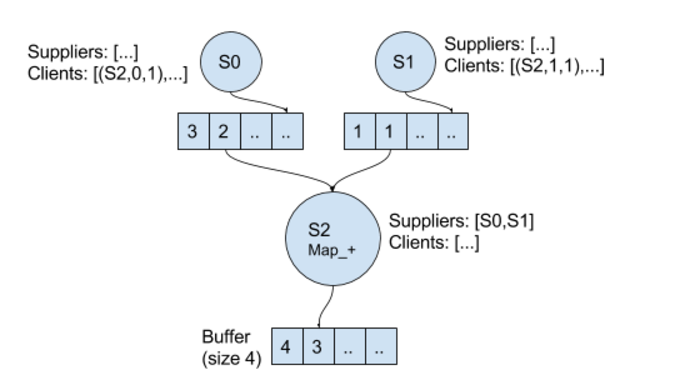
\includegraphics[width=0.9\linewidth]{fig/process}
	\caption{A process S2 of Xducer $\map{+}$. 
		It has read a 2 from S0's buffer and a 1 from S1's buffers, and it is writing a 3 to its own buffer.}
	\label{fig:process}
\end{figure}

The Xducer inside a process is the action-performing unit. 
We classify the atomic actions of a Xducer into three:
\begin{itemize}
	\item \pin: read one element from one supplier's buffer.
	\item \pout : write one element to its own buffer.
	\item \done: shutdown itself, no read or write any more.
\end{itemize}

A Xducer's actions can be considered as a sequential list of these three atomics.
For example,  the $\map{+}$ Xducer's action will be repetitions of two \pin s (reads from two suppliers respectively) followed by one \pout, and 
a \done \ action can be added where the Xducer should shutdown:
$$[\pin_0, \pin_1, \pout, \pin_0, \pin_1, \pout,... ,\done]$$
 where the subscripts of \pin indicate reading from different suppliers.

As discussed before, the Xducer knows when to shut itself down, that is, when it reads an EOS from the control stream. 
A process is responsible for providing the Xducer with the data and arranging the generated data into the buffer. 

The activities of a process is described as the following table shows.


 \begin{table}[H]\large
 	\renewcommand\arraystretch{1.5}
 	\centering
 	\begin{tabular}{|l|p{0.3\columnwidth}|p{0.3\columnwidth}|l|}  
 		\hline
 		 \diagbox{Xducer \\ action}{Buffer \\ state} & \filling & \draining \texttt{F} & \draining \texttt{T} \\ \hline
 		\pin  & \texttt{process-read}  & \texttt{process-read}; \texttt{allread-check}  & impossible \\
 		\hline
 		\pout &  write one element to buffer;
 		if buffer is full, switch to \draining \texttt{F}    &    enter write-block; \texttt{allread-check}   & impossible \\ 
 		\hline
 		\done &  switch to \draining \texttt{T}      & switch to \draining \texttt{T}   & \texttt{skip}  \\ 
 		\hline
 	\end{tabular}
 \caption{Process actions}
 \end{table}

\texttt{process-read}:

\begin{itemize}
	\item if the supplier's buffer state is \draining, and the read-cursor shows the process has not yet read all the data, then the process reads one element successfully and increases the read-cursor by one
	\item if the supplier's buffer state is \draining, but the read-cursor shows the process has read all the data, or the supplier's buffer state is \filling, then the process enters a read-block state
\end{itemize}

%full-check: if the buffer is full, switch it to \draining \texttt{F} state.

\texttt{allread-check}: if all the clients have read all the data of the buffer, switch it to \filling state.


\subsection{Scheduling}
The streaming execution model consists of two phases:
\begin{enumerate}[(1)]
\item Initialization \\
In this phase, the interpreter establishes the initial DAG by traversing the SVCODE program. The cases are:
\begin{itemize}
	\item initialize a sole stream definition $\sdef{s}{\lcall(s_1,...,s_k)}$: \\
	This is to set up one process $\s$:
	\begin{itemize}
		\item set its suppilers $\S$ = $[s_1,...,s_k]$
		\item add itself to its suppliers' $\clis$ with the corresponding channel number $\in \{1,...,k\}$ and a read-cursor number 0
		\item empty buffer of state \filling
		\item set up the specific Xducer $\lcall$
	\end{itemize}

	
	\item initialize a function call  $\scall{f}{[s_1,...,s_n]}{[s_1',...,s_m']}$: \\
	A user-defined function at runtime can be considered as another DAG, whose nodes(processes) of the formal arguments are missing. 
	So the interpreter just adds the function's DAG to the main program's DAG 
	and replaces the function's formal arguments with the actual parameters $[s_1,...,s_n]$, and the formal return ones with the actual ones $[s_1',...,s_m']$.  

	
	\item initialize a \wc block $\withctrl{\s_c}{p}{\Sin}{\Sout}$ \\
	At the initialization phase, the interpreter does not unfold $p$; instead, it mainly does the following two tasks:	
	\begin{itemize}
		\item prevents all the import streams of $\Sin$ from producing one more chunk (a full buffer) of data before the interpreter knows whether $s_c$ is an empty stream or not, i.e., add all of them a dummy client that never reads the buffer 
		\item initializes all the export streams of $\Sout$ as dummy processes that do not produce any data
	\end{itemize}

\end{itemize}


\item Loop scheduling. \\ 
This phase is a looping procedure. The condition of its end is that all the Xducers have shutdown, and all the buffers are in $\draining \T$ state. 

In a single scheduling round, the processes on the DAG are activated one by one from small to large.
The active process acts as we have seen in Table~\ref{fig:process} shows, until it enters a read-block or write-block state, or it is skipped.  
The results collected from each round consist the entire streams of the final result.

As long as a real (not dummy) process has been set up, it will keep working until its Xducer shutdown (although it may pause for some rounds due to read or write block). 
The crucial task in each round is to judge whether to unfold a \wc block or not. The judgment depends on the buffer state of the new control stream:

\begin{itemize}
	\item \filling$\emptyv$: the new control process has not produce any data yet, so the decision cannot be made in this round, thus delayed to the next round
	\item \draining$\emptyv \ \T$ : the new control stream is empty, thus no need to unfold the code, just set the export list streams also empty, and performs some other necessary clean-up job  
	\item other cases: the new control stream must be nonempty, thus the interpreter can unfold the code block now
\end{itemize}







	
\end{enumerate}

\subsection{Cost model}
Since we have defined the atomic actions of Xducers, it is now easy to define the low-level cost:
\begin{description}
	\item[Work] = the total number of \pin and \pout \  of all processes
	\item[Step] = the total number of switches from \filling to \draining of all processes
\end{description}


\subsection{Recursion}

In SVCODE, a recursive function call happens when the function body of $f$ from the instruction $\scall{f}{s_1,...,s_k}{(s_1',...,s'_{k'})}$ includes another \sc of  $f$.


For a non-recursive \sc, the effect of interpreting this instruction is almost transparent. 
For a recursive one, there is not much difference except one crucial point: the recursive \sc must be wrapped by a \wc block, otherwise it can never terminate.
At each time of interpreting an inline \sc, the function body is unfolded, but the \wc instruction inside it will stop it from further unfolding, that is, the stack-frame number only increases by one. 

At the high level, a SNESL program should use some conditional to decide when to terminate the recursion. 
As the only conditional of SNESL is the restricted comprehension, which is always translated to a \wc block wrapping the expression body,
so a recursion that can terminate at the high level will also terminate at the low level. 


\begin{example}
\end{example}
\begin{lstlisting}[style=nesl-style]
  -- define a function to compute factorial
  > function fact(x:int):int = if x <= 1 then 1 else x*fact(x-1)
  
  -- running example
  > {{fact(y): y in &x} : x in {5,10}}
  {{1,1,2,6,24},{1,1,2,6,24,120,720,5040,40320,362880}} :: {{int}}
\end{lstlisting}


% The function body of  \texttt{fact}:
%\lstinputlisting[style=svcode-style]{code/fact.svcode}

%TODO fix code
The translated SVCODE of the expression:
\lstinputlisting[style=svcode-style]{code/fact1.svcode}



\subsection{Deadlock}
An inherent tough issue of the streaming execution model is the risk of deadlock, which is mainly due to the limitation of available memory and the irreversibility (maybe ?) of time.
In general, we classify deadlock situations into two types: soft deadlock, which can be broken not necessarily by enlarging the buffer size, and hard deadlock, which can only be solved by enlarging the buffer size. 

\begin{itemize}

\item Soft deadlock: \\

One case of soft deadlock can be due to the different data rates of processes that leads to a situation where some buffer(s) of $\filling$ state can never turn to \draining. 
For example, the following expression tries to negate the elements that can be divided by 5 exactly of a sequence.
\begin{example}\emph{ A soft deadlock that can be broken by stealing}
\end{example}
\begin{lstlisting}[style=nesl-style]
  -- buffer size 4 
 > concat({{-x | x % 5 == 0} ++ {x | x %5 != 0} :  x in &10})
 {0,1,2,3,4,-5,6,7,8,9} :: {int}
\end{lstlisting}

% TODO draw picture 
% text not good
In this example, the argument sequence contains elements from 0 to 9; the subsequence of the negated numbers, containing only 0 and -5, are concatenated with the one of the other eight numbers. 
Since these two subsequences are generated at different rates,
the buffer for holding the shorter subsequence cannot get full when the other for the longer subsequence is already full to drain.
Then the Xducer for appending their elements deadlocks.
But if we minimize the buffer size to 1, then the deadlock can be broken, since buffer of size one can always turn to \draining mode as long as there is one element generated. 

In our implementation, we use a $stealing$ strategy to  automatically avoid this type of deadlock. 
The idea is that when a deadlock is detected, we will first switch the smallest process with a \filling buffer into \draining mode to see if the deadlock can be broken; if not, we repeat this switch until the deadlock is broken; or otherwise, it may be a hard deadlock.

Since the stealing strategy is basically a premature
switch from \filling to \draining, the low-level step cost is possible to be affected and the effect depends on the concrete program and the buffer size. 
Some future work can be further investigation about the effect of this stealing strategy on the cost model.\\


\item Hard deadlock: \\
This type of deadlock is mainly because of insufficient space.

One case of soft deadlock can be caused by trying to traverse the same sequence multiple times. 

\begin{example} \emph{A soft deadlock caused by travesing the sequence $x$ two times.} \label{eg:deadlock1}
\end{example}
\begin{lstlisting}[style=nesl-style]
> let x = {1} in x ++ x
Deadlock!
\end{lstlisting}

There are at least two feasible solutions to this case.
One is manually rewriting the code to define new variables for the same sequence, as the following code shows :\\

\begin{lstlisting}[style=nesl-style]
> let x = {1}; y = {1} in x ++ y
{1,1} :: {int}
\end{lstlisting}

The other can be done by optimizing the compiler to support multi-traversing check and automatic 
redefinition of retraversed sequences, or other possible methods. 
As the code grows more complicated, locating the problem can become much harder, thus a smarter compiler is definitely necessary. 
This is worth some future investigation.\\


\begin{example} \emph{The following SNESL function {\ttfamily oeadd} risks a hard deadlock. Given an integer sequence with an equal number of odd and even elements, this function will try to perform addition on a pair of odd and even number with the same index in their respective subsequences.} 
\end{example}

\lstinputlisting[style=nesl-style]{code/harddeadlock.snesl} 
\hspace{0.3cm}

If we give the function a proper argument, for example, an sequence of an odd and an even interleaving with each other, it will never deadlock, even with a buffer of size one. 
But if there is a relatively large distance between any odd-even pair, the code may deadlock.  \\
  
\begin{lstlisting}[style=nesl-style]
-- buffer size 1

> oeadd(&30)
{1,5,9,13,17,21,25,29,33,37,41,45,49,53,57} :: {int}

> oeadd({1,3,5,7,0,2,4,8})
Deadlock!
\end{lstlisting}

% TODO or recalculation
This type of deadlock may only be broken by enlarging the buffer size. 


\end{itemize}


%\subsection{[optional] Evaluation}
%Some possibilities for improving the scheduling:
%
%\begin{itemize}
%\item The processes in a block state will be activated in the next scheduling round, but it may still  block itself immediately since the blocking condition still holds. So a better strategy can be 
%
%\item The processes are activated only one by one, even though some of them can be data-independent, this simulates a SIMD machine execution. But it should be able to be optmized to support MIMD machine. 
%Evaluation of some high-level expressions, such as the evaluation of the components of a tuple or a function call , can be executed in parallel as well.
%

%\end{itemize}

\subsection{Examples}


\lstinputlisting[style=nesl-style]{code/uc_scanred.snesl}

\begin{lstlisting}[style=nesl-style]
-- buffer size 1
> scanred(&16,16)
({0,0,1,3,6,10,15,21,28,36,45,55,66,78,91,105},120) :: ({int},int)
\end{lstlisting}
